%!TEX root = ../talk.tex

\section{Python}\label{sec:python}

%%%
\subsection{A short introduction on Python}
%%%

\begin{frame}
  \MyLogo
  \frametitle{Python: A general-purpose programming language}  

\small 

\begin{itemize}

\item Created by Guido van Rossum in 1989 and first released in 1991

\item Named after ``the Monty Python'' (British comedy group)

\item An interpreted language---simple, clear, and readable 

\item Python has many excellent packages for machine learning

\item The language of choice in introductory programming courses

\end{itemize}

\begin{figure}[htbp] %  figure placement: here, top, bottom, or page
   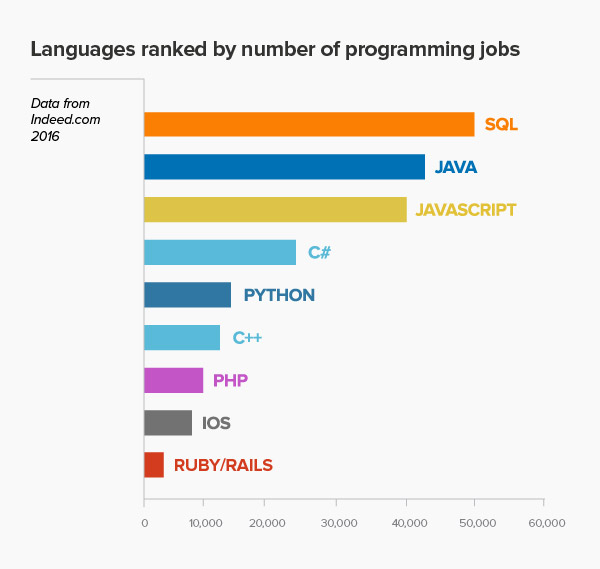
\includegraphics[height=1.7in]{figures/ComputerLanguagesDemand.jpg} 
   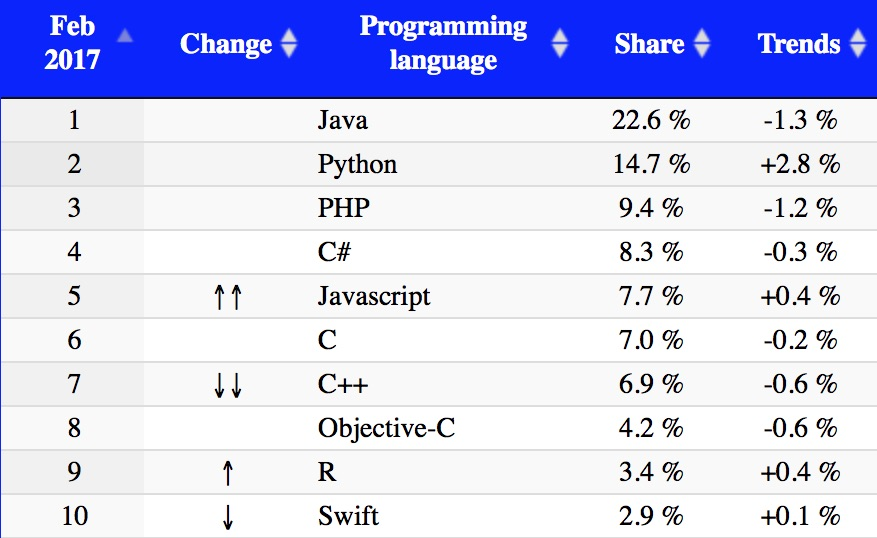
\includegraphics[height=1.7in]{figures/ComputerLanguagesShare.jpg} 
\end{figure}

\end{frame}

%%%

\begin{frame}
  \MyLogo
  \frametitle{Python for Scientific Computing}  

\small

\structure{Why Python for scientific computing?}
\begin{itemize}
	\item Strong introspection\footnote {Code introspection is the ability to examine classes, functions and keywords to know what they are, what they do and what they know.Python provides several functions and utilities for code introspection, like dir(), help(), type().} capabilities (???What does even mean???)
	
	\item Full modularity, supporting hierarchical packages
	\item Exception-based error handling
	\item Dynamic data types and automatic memory management
\end{itemize}

\structure{Why consider such a slow language for simulation?}
\begin{itemize}
	\item Good for proof-of-concept
	\item Implementation time versus execution time
	\item Code readability and maintenance --- short code, fewer bugs
	\item Well-written Python code is ``fast enough'' for most computational tasks
	\item Time critical parts executed through compiled language or \alert{available packages}
\end{itemize}

\end{frame}

%%%
\subsection{Basic language components}
%%%

\begin{frame}[fragile]
  \MyLogo
  \frametitle{Built-in Data Structures}  
\small

\begin{itemize}
	\item[$\bullet$] Numeric types--int, float, complex
	\begin{lstlisting}[language=python]
	For example:
	a=1 int
	b=1.0 float
	c=1L long int
	d=0xf int(hex format)
	e=010 int(octal format)
	f=1+2j complex
	\end{lstlisting}

	\item[$\bullet$] Sequence types--list, tuple, str, dict
	\begin{lstlisting}[language=python]
	For example:
	g=[3.14, True, 'Yes', [1], (1L,)] + [None]*3, list
	h=(3.14, True, 'Yes', [1], ()), tuple
	i='Hello' + "," + '''world!''', str
	j=\{1: 'int', 'pi': 3.14\}, dict
	\end{lstlisting}
\end{itemize}
\end{frame}

%%%

\begin{frame}[fragile]
  \MyLogo
  \frametitle{Control Flow}  
\small

\begin{itemize}
	\item[$\bullet$] If-then-else
	\begin{lstlisting}[language=python]
		a = 1
		if a > 0:
			print "a is positive"
		elif a=0:
			print "a is zero"
		else:
			print "a is negative"
	\end{lstlisting}			
	\item[$\bullet$] For loop
	\begin{lstlisting}[language=python]
		for i in range(10):
			print i
	\end{lstlisting}	
	\item[$\bullet$] While loop
	\begin{lstlisting}[language=python]
		sum = 0; i = 0
		while i < 10:
			sum += i
			i += 1
	\end{lstlisting}
\end{itemize}

\end{frame}

%%%

\begin{frame}[fragile]
  \MyLogo
  \frametitle{Functions and Modules}  
\small

\begin{itemize}
	\item[$\bullet$] Defining functions 
		\begin{lstlisting}[language=python]
			def square(x):
				return x*x
		\end{lstlisting}		
	\item[$\bullet$] Using modules\\
			There are 3 different ways to use modules. Examples are below.\\
			1. import math\\
				This will only introduce the name math into the name space in which the import command was issued. The names within the math module will not appear in the enclosing namespace: they must be accessed through the name math. For example: math.sin(3.14).\\
			2. from math import *\\
				This does not introduce the name math into the current namespace. It does however introduce all public names of the math module into the current namespace, directly using: sin(3.14)\\
			3. from math import sin\\
				This will only import the sin function from math module and introduce the name sin into the current namespace, but it will not introduce the name math into the current namespace, directly using: sin(3.14)
		
\end{itemize}

\end{frame}
